\documentclass[12pt,letterpaper]{article}
\usepackage{pgf}
\usepackage{amsmath,amsthm,amsfonts,amssymb,amscd}
\usepackage{fullpage}
\usepackage{lastpage}
\usepackage{enumerate}
\usepackage{fancyhdr}
\usepackage{mathrsfs}
\usepackage{xcolor}
\usepackage{graphicx}
\usepackage{color}
\usepackage[margin=3cm]{geometry}
\setlength{\parindent}{0.0in}
\setlength{\parskip}{0.05in}

\sloppy
\definecolor{lightgray}{gray}{0.5}
\setlength{\parindent}{0pt}

% Edit these as appropriate
\newcommand\course{20CS6037}
\newcommand\semester{Fall 2014}     % <-- current semester
\newcommand\hwnum{3}                  % <-- homework number
\newcommand\yourname{Khaldoon Alshouiliy, Kyungmook Park } % <-- your name
\newcommand\login{M06967001, M07068980}           % <-- your NetID
\newcommand\hwdate{Due: 11:59PM 10/20/2014}           % <-- HW due date

\newenvironment{answer}[1]{
  \subsubsection*{Problem #1}
}


\pagestyle{fancyplain}
\headheight 35pt
\lhead{\yourname\ \login\\\course\ --- \semester}
\chead{\textbf{\Large Homework \hwnum}}
\rhead{\hwdate}
\headsep 10pt

\begin{document}

\noindent \emph{Homework Notes:} Hours spent on this HW: ~14 hours. It took fairly long to figure out debugging the code and understand how to measure overlap.

\section*{Versicolor VS Virginica and Setosa}

    \begin{verbatim}
close all;
clear all;
load('fisheriris');
[r, c]=size(meas);
% Extend meas by 1 to account for the bias
col1 = ones(r,1);
emeas=[col1 meas];

%Assign numerical labels
for i=1:50, class(i)=1; end %setosa
for i=51:100, class(i)=2; end %versicolor
for i = 101:150, class(i) = 3; end %virginica
%Transform numerical lables into 0 / 1 labels
newclass(class==1) = 0; %setosa becomes class 0%
% the rest are in class 1
newclass(class == 2) = 1;
newclass(class == 3) = 1;
p = 0.1; % extent of training sets
randindex=randperm(r);
N = round(p*r)
train = emeas(randindex(1:N),:);
trainlabels = newclass(randindex(1:N));
test = emeas(randindex(N+1:r),:);
testlabels = newclass(randindex(N+1:r));
%N = 15;

% initialize w
w=zeros(c+1,1);
w2=zeros(c+1,1);
ybar=mean(trainlabels);
w(1)=log(ybar/(1-ybar));
s=zeros(1,N);
z=zeros(N,1);

%Convergence Criterion
epsil = 2.2204e-16;
iter = 100000;
s0 = 0;

%Alg 8.2

%Signmoid function

%mui = exp(mu) / (exp(mu) + 1);


for i = 1:iter,

    eta = w(1) + train * w;
    mu = exp(eta) ./ (exp(eta) + 1);
    s = mu.*(1-mu);
    z = eta + (trainlabels'-mu) ./ s;
    S = diag(s);

    fprintf('The value of s is %d.\n',s(1))
    fprintf('The iteration number is %d.\n',i)

    %Calculate the difference between previous and current s
    sDiff = S(1) - s0;
    if (sDiff < epsil),
        fprintf('The value of s is %d.\n',s(1))
        fprintf('Converged in %d steps\n',i)
        break;
    end

    s0 = S(1);
    w = inv(train'*S*train)*train'*S*z;

end


%Test

ltest=length(testlabels);
% Compute the output for each test data using w
for i=1:ltest,
out(i)=test(i,:)*w;
end
% Transform output in 0 1 labels
out1=out;
out1(out<0)=0;
out1(out>0)=1;
% compute accuracy
accuracy = 1 - sum(abs(testlabels - out1))/ltest
%plot ROC curves
figure
plotroc(testlabels, out1);
% plot confusion matrix
figure
plotconfusion(testlabels, out1);
\end{verbatim}

        \color{lightgray} \begin{verbatim}
N =

    15

The value of s is 2.455948e-01.
The iteration number is 1.
The value of s is 5.355942e-02.
The iteration number is 2.
The value of s is 5.355942e-02.
Converged in 2 steps

accuracy =

     1

\end{verbatim} \color{black}
    
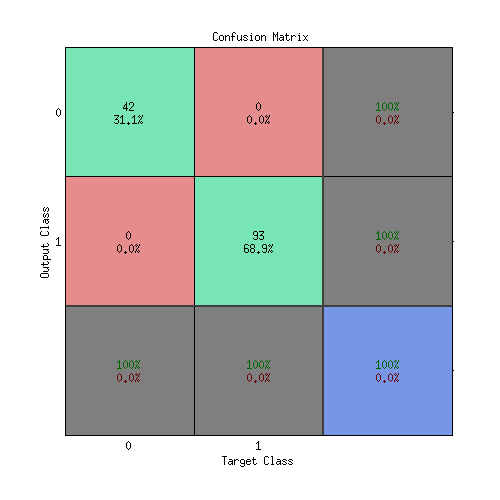
\includegraphics [width=4in]{VersicolorVsVirginicaAndSetosa_ConfusionMatrix.png}

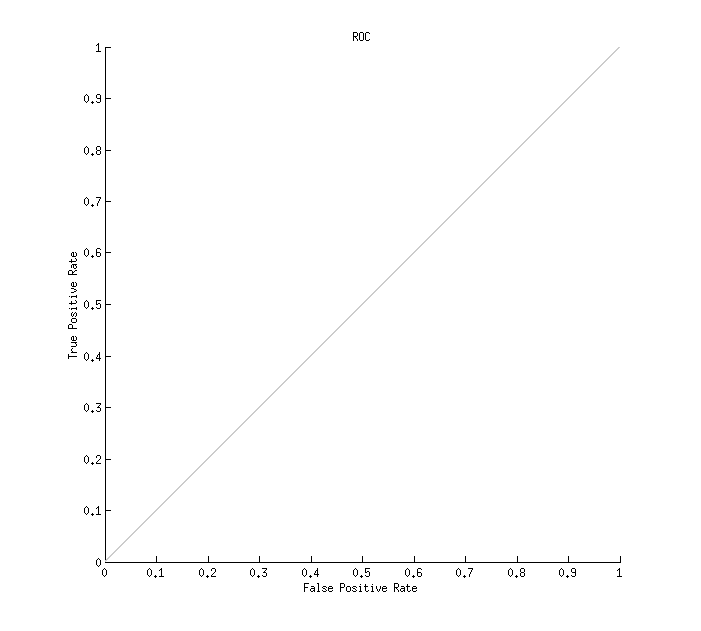
\includegraphics [width=4in]{VersicolorVsVirginicaAndSetosa_ROC.png}

\section*{Setosa VS Virginica and Versicolor}

\textbf{MatLab Answer}

    \begin{verbatim}
close all;
clear all;
load('fisheriris');
[r, c]=size(meas);
% Extend meas by 1 to account for the bias
col1 = ones(r,1);
emeas=[col1 meas];

%Assign numerical labels
for i=1:50, class(i)=1; end %setosa
for i=51:100, class(i)=2; end %versicolor
for i = 101:150, class(i) = 3; end %virginica
%Transform numerical lables into 0 / 1 labels
newclass(class==1) = 1; %setosa becomes class 0%
% the rest are in class 1
newclass(class == 2) = 0;
newclass(class == 3) = 1;
p = 0.1; % extent of training sets
randindex=randperm(r);
N = round(p*r)
train = emeas(randindex(1:N),:);
trainlabels = newclass(randindex(1:N));
test = emeas(randindex(N+1:r),:);
testlabels = newclass(randindex(N+1:r));
%N = 15;

% initialize w
w=zeros(c+1,1);
w2=zeros(c+1,1);
ybar=mean(trainlabels);
w(1)=log(ybar/(1-ybar));
s=zeros(1,N);
z=zeros(N,1);

%Convergence Criterion
epsil = 2.2204e-16;
iter = 10000000;
s0 = 0;

%Alg 8.2

%Signmoid function

%mui = exp(mu) / (exp(mu) + 1);


for i = 1:iter,

    eta = w(1) + train * w;
    mu = exp(eta) ./ (exp(eta) + 1);
    s = mu.*(1-mu);
    z = eta + (trainlabels'-mu) ./ s;
    S = diag(s);

    fprintf('The value of s is %d.\n',s(1))
    fprintf('The iteration number is %d.\n',i)

    %Calculate the difference between previous and current s
    sDiff = S(1) - s0;
    if (sDiff < epsil),
        fprintf('The value of s is %d.\n',s(1))
        fprintf('Converged in %d steps\n',i)
        break;
    end

    s0 = S(1);
    w = inv(train'*S*train)*train'*S*z;

end


%Test

ltest=length(testlabels);
% Compute the output for each test data using w
for i=1:ltest,
out(i)=test(i,:)*w;
end
% Transform output in 0 1 labels
out1=out;
out1(out<0)=0;
out1(out>0)=1;
% compute accuracy
accuracy = 1 - sum(abs(testlabels - out1))/ltest
%plot ROC curves
figure
plotroc(testlabels, out1);
% plot confusion matrix
figure
plotconfusion(testlabels, out1);
\end{verbatim}

        \color{lightgray} \begin{verbatim}
N =

    15

The value of s is 2.455948e-01.
The iteration number is 1.
The value of s is 3.246542e-03.
The iteration number is 2.
The value of s is 3.246542e-03.
Converged in 2 steps

accuracy =

    0.6296

\end{verbatim} \color{black}

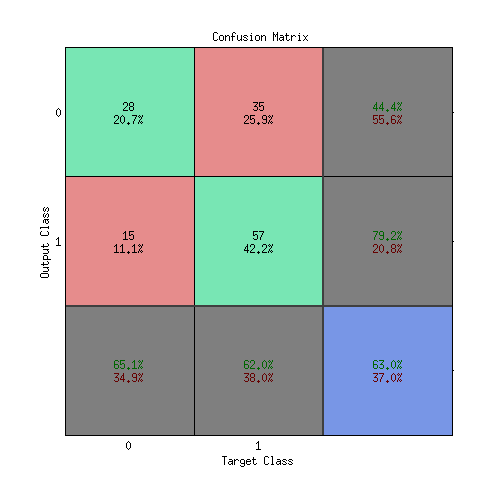
\includegraphics [width=4in]{HW3_SetVirandVerCM.png}

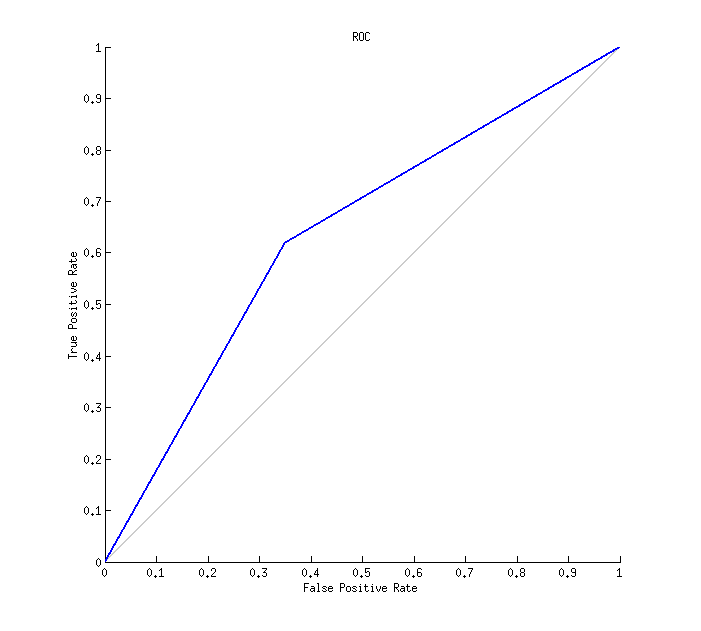
\includegraphics [width=4in]{HW3_SetVirandVerROC.png}

Overlap occurs when there two classes collide within the data space. Any missed class on the confusion matrix can be measured as a frequency of overlap, i.e. 0.259 + 0.111 $= $ 0.37  in this case.

\section*{Virginica vs Setosa and Versicolor}

    \begin{verbatim}
close all;
clear all;
load('fisheriris');
[r, c]=size(meas);
% Extend meas by 1 to account for the bias
col1 = ones(r,1);
emeas=[col1 meas];

%Assign numerical labels
for i=1:50, class(i)=3; end %setosa
for i=51:100, class(i)=2; end %versicolor
for i = 101:150, class(i) = 1; end %virginica
%Transform numerical lables into 0 / 1 labels
newclass(class==1) = 1; %setosa becomes class 0%
% the rest are in class 1
newclass(class == 2) = 0;
newclass(class == 3) = 1;
p = 0.1; % extent of training sets
randindex=randperm(r);
N = round(p*r)
train = emeas(randindex(1:N),:);
trainlabels = newclass(randindex(1:N));
test = emeas(randindex(N+1:r),:);
testlabels = newclass(randindex(N+1:r));
%N = 15;

% initialize w
w=zeros(c+1,1);
w2=zeros(c+1,1);
ybar=mean(trainlabels);
w(1)=log(ybar/(1-ybar));
s=zeros(1,N);
z=zeros(N,1);

%Convergence Criterion
epsil = 2.2204e-16;
iter = 10000000;
s0 = 0;

%Alg 8.2

%Signmoid function

%mui = exp(mu) / (exp(mu) + 1);


for i = 1:iter,

    eta = w(1) + train * w;
    mu = exp(eta) ./ (exp(eta) + 1);
    s = mu.*(1-mu);
    z = eta + (trainlabels'-mu) ./ s;
    S = diag(s);

    fprintf('The value of s is %d.\n',s(1))
    fprintf('The iteration number is %d.\n',i)

    %Calculate the difference between previous and current s
    sDiff = S(1) - s0;
    if (sDiff < epsil),
        fprintf('The value of s is %d.\n',s(1))
        fprintf('Converged in %d steps\n',i)
        break;
    end

    s0 = S(1);
    w = inv(train'*S*train)*train'*S*z;

end


%Test

ltest=length(testlabels);
% Compute the output for each test data using w
for i=1:ltest,
out(i)=test(i,:)*w;
end
% Transform output in 0 1 labels
out1=out;
out1(out<0)=0;
out1(out>0)=1;
% compute accuracy
accuracy = 1 - sum(abs(testlabels - out1))/ltest
%plot ROC curves
figure
plotroc(testlabels, out1);
% plot confusion matrix
figure
plotconfusion(testlabels, out1);
\end{verbatim}

        \color{lightgray} \begin{verbatim}
N =

    15

The value of s is 2.455948e-01.
The iteration number is 1.
The value of s is 6.566867e-02.
The iteration number is 2.
The value of s is 6.566867e-02.
Converged in 2 steps

accuracy =

    0.6000

Overlap occurs when there two classes collide within the data space. Any missed class on the confusion matrix can be measured as a frequency of overlap, i.e. 0.4  in this case.

\end{verbatim} \color{black}
    
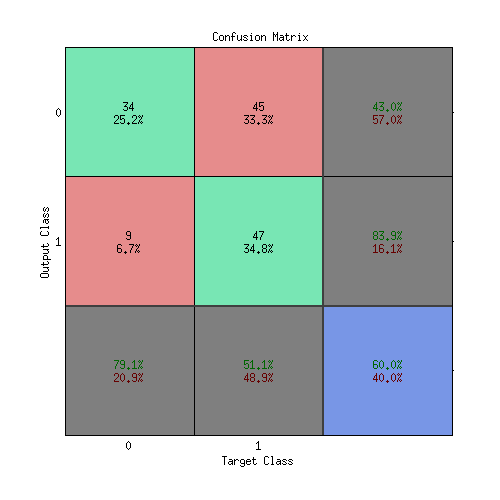
\includegraphics [width=4in]{HW3_ViSVerCM.png}

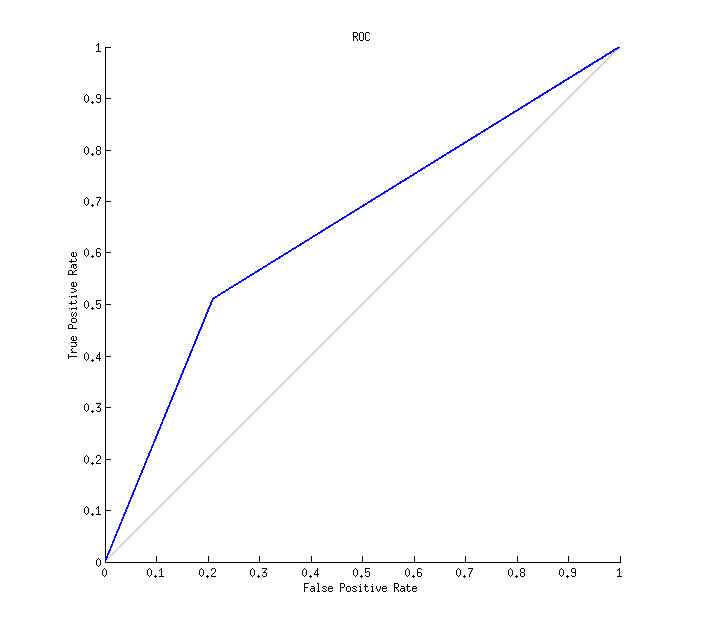
\includegraphics [width=4in]{HW3_ViSVerROC.png}

\section*{Versicolor vs Setosa and Virginica}

    \begin{verbatim}
close all;
clear all;
load('fisheriris');
[r, c]=size(meas);
% Extend meas by 1 to account for the bias
col1 = ones(r,1);
emeas=[col1 meas];

%Assign numerical labels
for i=1:50, class(i)=2; end %setosa
for i=51:100, class(i)=1; end %versicolor
for i = 101:150, class(i) = 3; end %virginica
%Transform numerical lables into 0 / 1 labels
newclass(class==1) = 1; %setosa becomes class 0%
% the rest are in class 1
newclass(class == 2) = 1;
newclass(class == 3) = 0;
p = 0.1; % extent of training sets
randindex=randperm(r);
N = round(p*r)
train = emeas(randindex(1:N),:);
trainlabels = newclass(randindex(1:N));
test = emeas(randindex(N+1:r),:);
testlabels = newclass(randindex(N+1:r));
%N = 15;

% initialize w
w=zeros(c+1,1);
w2=zeros(c+1,1);
ybar=mean(trainlabels);
w(1)=log(ybar/(1-ybar));
s=zeros(1,N);
z=zeros(N,1);

%Convergence Criterion
epsil = 2.2204e-16;
iter = 10000000;
s0 = 0;

%Alg 8.2

%Signmoid function

%mui = exp(mu) / (exp(mu) + 1);


for i = 1:iter,

    eta = w(1) + train * w;
    mu = exp(eta) ./ (exp(eta) + 1);
    s = mu.*(1-mu);
    z = eta + (trainlabels'-mu) ./ s;
    S = diag(s);

    fprintf('The value of s is %d.\n',s(1))
    fprintf('The iteration number is %d.\n',i)

    %Calculate the difference between previous and current s
    sDiff = S(1) - s0;
    if (sDiff < epsil),
        fprintf('The value of s is %d.\n',s(1))
        fprintf('Converged in %d steps\n',i)
        break;
    end

    s0 = S(1);
    w = inv(train'*S*train)*train'*S*z;

end


%Test

ltest=length(testlabels);
% Compute the output for each test data using w
for i=1:ltest,
out(i)=test(i,:)*w;
end
% Transform output in 0 1 labels
out1=out;
out1(out<0)=0;
out1(out>0)=1;
% compute accuracy
accuracy = 1 - sum(abs(testlabels - out1))/ltest
%plot ROC curves
figure
plotroc(testlabels, out1);
% plot confusion matrix
figure
plotconfusion(testlabels, out1);
\end{verbatim}

        \color{lightgray} \begin{verbatim}
N =

    15

The value of s is 2.455948e-01.
The iteration number is 1.
The value of s is 2.472695e-07.
The iteration number is 2.
The value of s is 2.472695e-07.
Converged in 2 steps

accuracy =

    0.8593

\end{verbatim} \color{black}
    
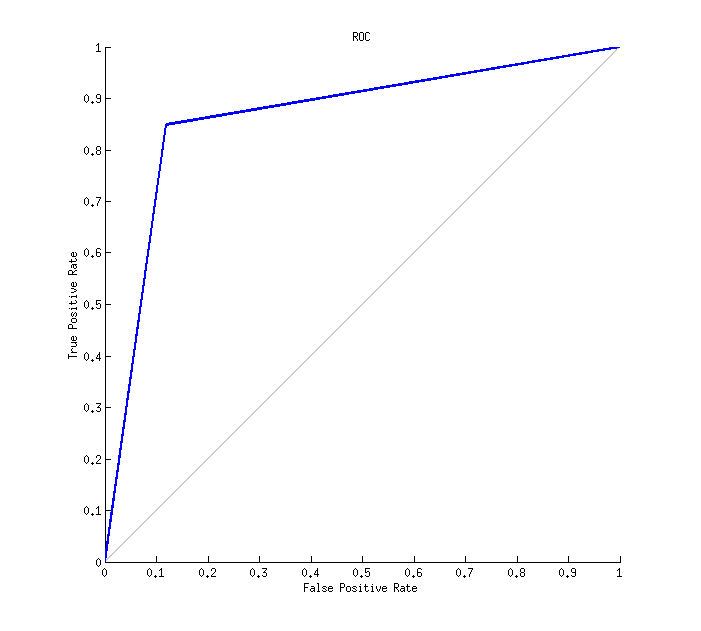
\includegraphics [width=4in]{HW3_VSViROC.png}

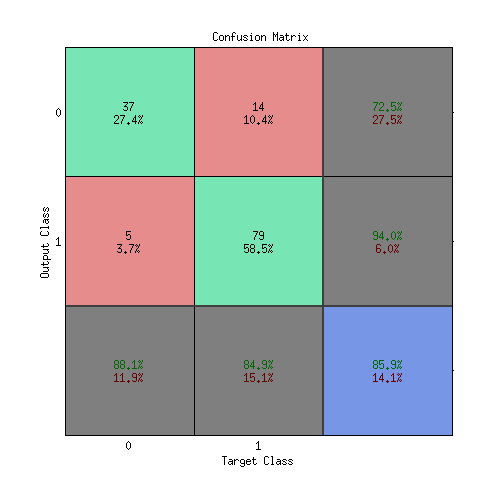
\includegraphics [width=4in]{HW3_VSViCM.png}

Overlap occurs when there two classes collide within the data space. Any missed class on the confusion matrix can be measured as a frequency of overlap, i.e. 0.14  in this case.

\end{document}
    


\end{document}
